
\begin{figure}
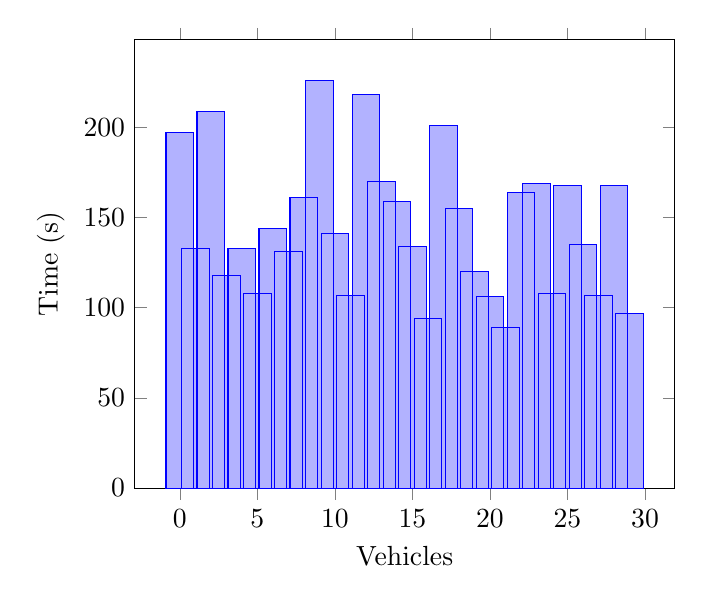
\begin{tikzpicture}
\begin{axis}[
legend style={anchor=west},
xlabel=Vehicles,
ylabel=Time (s),
ymin=0,
ybar,
]
\addplot coordinates {
(0, 197)
(1, 133)
(2, 209)
(3, 118)
(4, 133)
(5, 108)
(6, 144)
(7, 131)
(8, 161)
(9, 226)
(10, 141)
(11, 107)
(12, 218)
(13, 170)
(14, 159)
(15, 134)
(16, 94)
(17, 201)
(18, 155)
(19, 120)
(20, 106)
(21, 89)
(22, 164)
(23, 169)
(24, 108)
(25, 168)
(26, 135)
(27, 107)
(28, 168)
(29, 97)
};

\end{axis}
\end{tikzpicture}
\label{tik:100:70}
\caption{100 percent diving with GSC on route $70$}
\end{figure}
